\documentclass[conference]{IEEEtran}

% --- Minimal packages for a stand-alone figures PDF ---
\usepackage{graphicx}
\usepackage{tikz}
\usepackage{pgfplots}
\pgfplotsset{compat=1.18}
\usetikzlibrary{arrows.meta,positioning,fit}

% (本文とは独立に)図表だけを並べる
\begin{document}
\title{Figures and Tables for ``FeFET CMOS 0.18~$\mu$m Integration Study''}
\author{}\maketitle

\section*{Figures and Tables}

% ================= Fig.1 : Process flow (TikZ) =================
\begin{figure}[!t]\centering
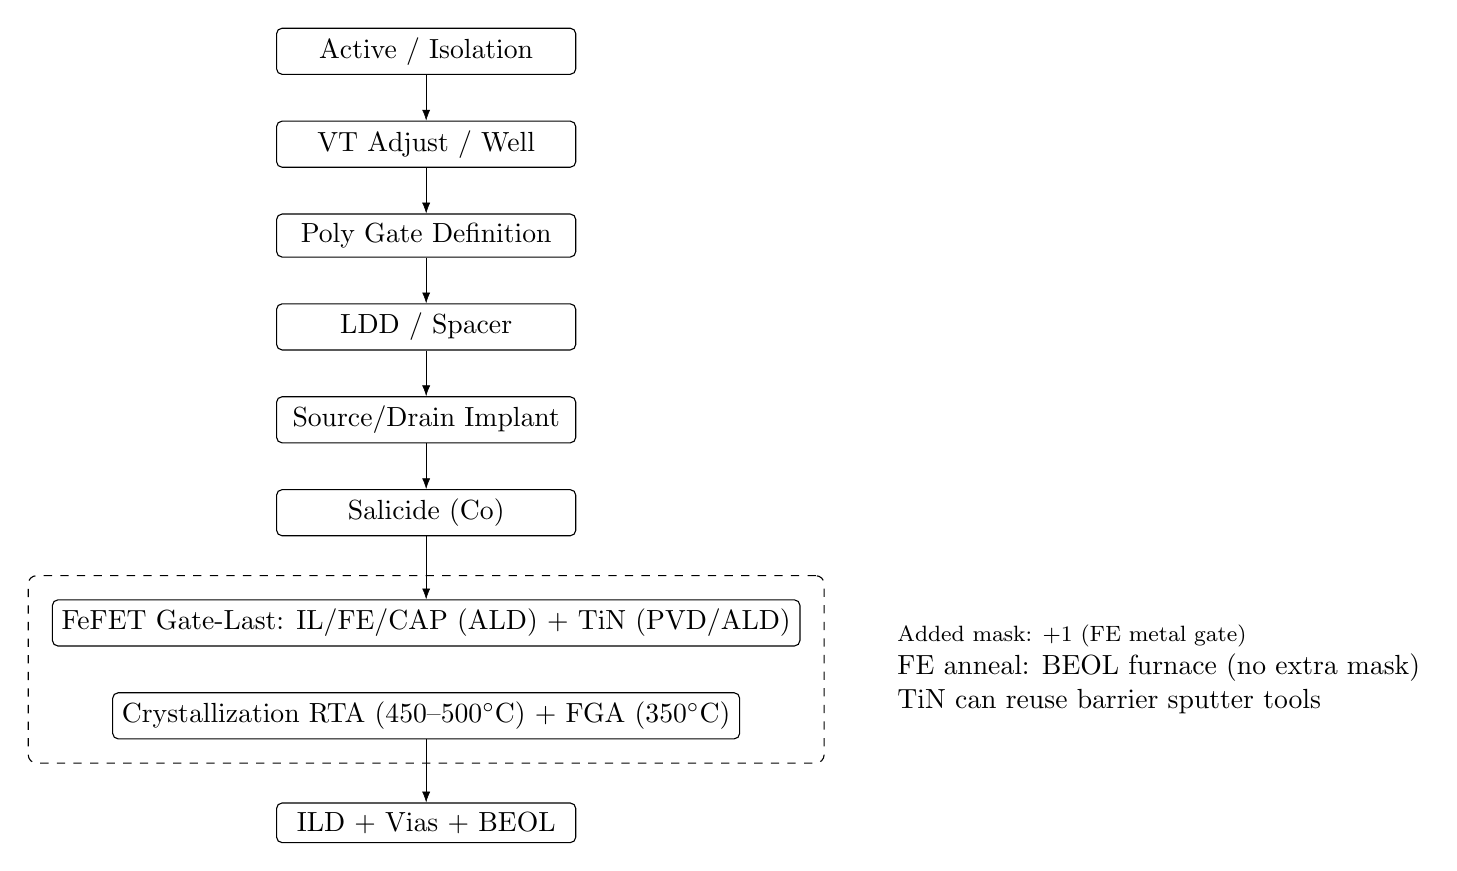
\begin{tikzpicture}[
  box/.style={draw, rounded corners=2pt, minimum width=38mm, minimum height=5mm},
  flow/.style={-Latex, very thin},
  node distance=5.8mm
]
% vertical flow blocks
\node[box] (n1) {Active / Isolation};
\node[box, below=of n1] (n2) {VT Adjust / Well};
\node[box, below=of n2] (n3) {Poly Gate Definition};
\node[box, below=of n3] (n4) {LDD / Spacer};
\node[box, below=of n4] (n5) {Source/Drain Implant};
\node[box, below=of n5] (n6) {Salicide (Co)};

% FeFET gate-last module (dashed region)
\node[box, below=8mm of n6] (g1) {FeFET Gate-Last: IL/FE/CAP (ALD) + TiN (PVD/ALD)};
\node[box, below=of g1] (g2) {Crystallization RTA (450--500$^\circ$C) + FGA (350$^\circ$C)};
\node[draw, dashed, rounded corners=3pt, fit=(g1)(g2), inner sep=3mm, label={[align=left]south east:}] (dregion) {};

% Continue to BEOL
\node[box, below=8mm of g2] (n7) {ILD + Vias + BEOL};

% vertical arrows
\foreach \a/\b in {n1/n2,n2/n3,n3/n4,n4/n5,n5/n6,n6/g1,g2/n7}
  \draw[flow] (\a.south) -- (\b.north);

% right notes
\node[align=left, anchor=west] (notes) at ([xshift=8mm]dregion.east) {%
\footnotesize Added mask: +1 (FE metal gate)\\
FE anneal: BEOL furnace (no extra mask)\\
TiN can reuse barrier sputter tools};

\end{tikzpicture}
\caption{Placement of the FeFET gate-last module within the 0.18~$\mu$m CMOS baseline (vertical layout).}
\end{figure}

% ================= Table I : Added mask =================
\begin{table}[!t]\centering
\caption{Added masks / process steps relative to baseline logic.}
\begin{tabular}{|c|c|l|}\hline
Step & Mask & Comment\\ \hline
FE metal gate & +1 & Reuse analog option route\\
FE anneal     & 0  & Performed in BEOL furnace (no extra mask)\\ \hline
\end{tabular}
\end{table}

% ================= Fig.2 : Endurance (pgfplots) =================
\begin{figure}[!t]\centering
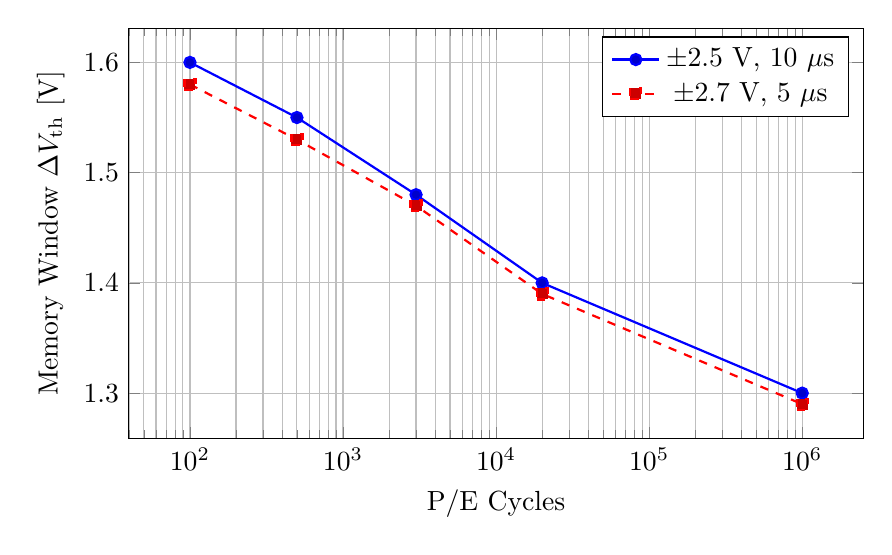
\begin{tikzpicture}
\begin{axis}[
  width=0.9\linewidth, height=0.56\linewidth,
  xlabel={P/E Cycles}, xmode=log, log basis x=10,
  ylabel={Memory Window $\Delta V_{\mathrm{th}}$ [V]},
  grid=both, tick label style={/pgf/number format/fixed}
]
  \addplot+[mark=*, thick] coordinates
    {(1e2,1.60) (5e2,1.55) (3e3,1.48) (2e4,1.40) (1e6,1.30)};
  \addlegendentry{$\pm 2.5$ V, 10 $\mu$s}

  \addplot+[mark=square*, dashed, thick] coordinates
    {(1e2,1.58) (5e2,1.53) (3e3,1.47) (2e4,1.39) (1e6,1.29)};
  \addlegendentry{$\pm 2.7$ V, 5 $\mu$s}
\end{axis}
\end{tikzpicture}
\caption{Schematic endurance behavior of HZO-FeFETs in a 0.18~$\mu$m flow.}
\end{figure}

% ================= Fig.3 : Wake-up + Retention (縦並び) =================
\begin{figure}[!t]\centering
% Wake-up (top)
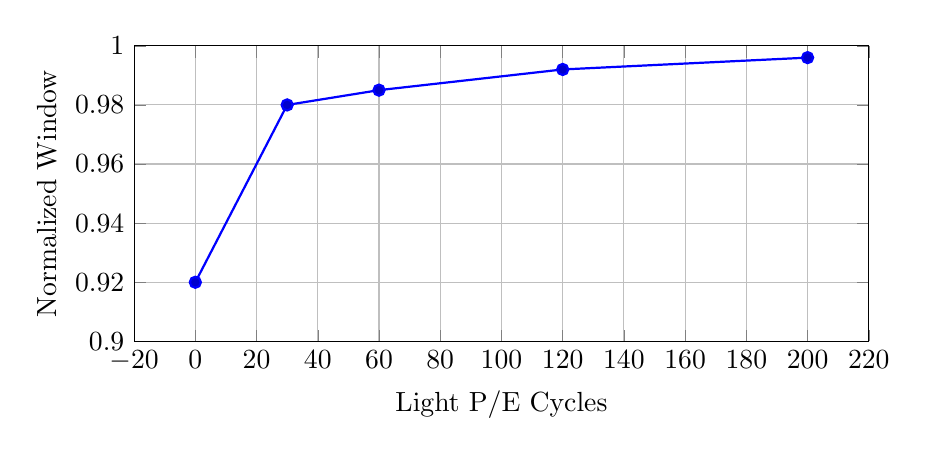
\begin{tikzpicture}
\begin{axis}[
  width=0.9\linewidth, height=0.44\linewidth,
  xlabel={Light P/E Cycles}, ylabel={Normalized Window},
  ymin=0.90, ymax=1.00, grid=both,
  tick label style={/pgf/number format/fixed}
]
  \addplot+[mark=*, thick] coordinates
    {(0,0.92) (30,0.98) (60,0.985) (120,0.992) (200,0.996)};
\end{axis}
\end{tikzpicture}

\vspace{0.6em}

% Retention (bottom)
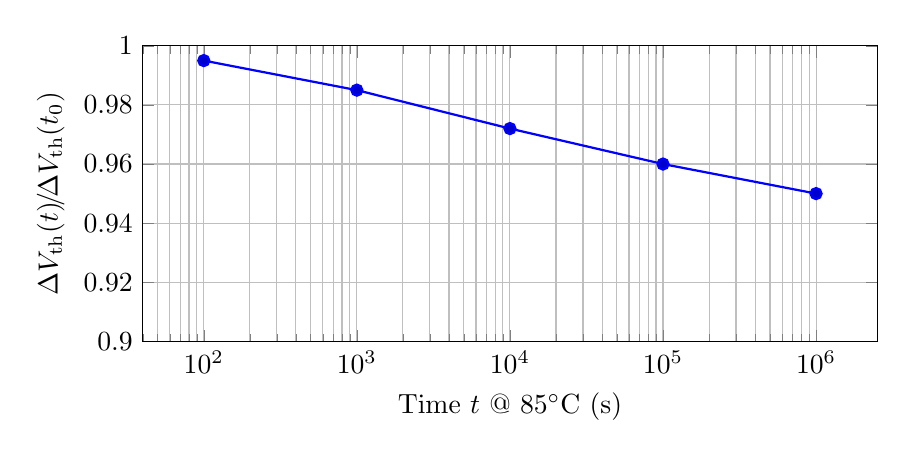
\begin{tikzpicture}
\begin{axis}[
  width=0.9\linewidth, height=0.44\linewidth,
  xmode=log, log basis x=10, grid=both,
  xlabel={Time $t$ @ 85$^\circ$C (s)}, ylabel={$ \Delta V_{\mathrm{th}}(t)\!/\!\Delta V_{\mathrm{th}}(t_0)$},
  ymin=0.90, ymax=1.00,
  tick label style={/pgf/number format/fixed}
]
  \addplot+[mark=*, thick] coordinates
    {(1e2,0.995) (1e3,0.985) (1e4,0.972) (1e5,0.960) (1e6,0.950)};
\end{axis}
\end{tikzpicture}
\caption{Wake-up (top) and retention projection at 85$^\circ$C (bottom).}
\end{figure}

% ================= Fig.4 : TDDB Weibull =================
\begin{figure}[!t]\centering
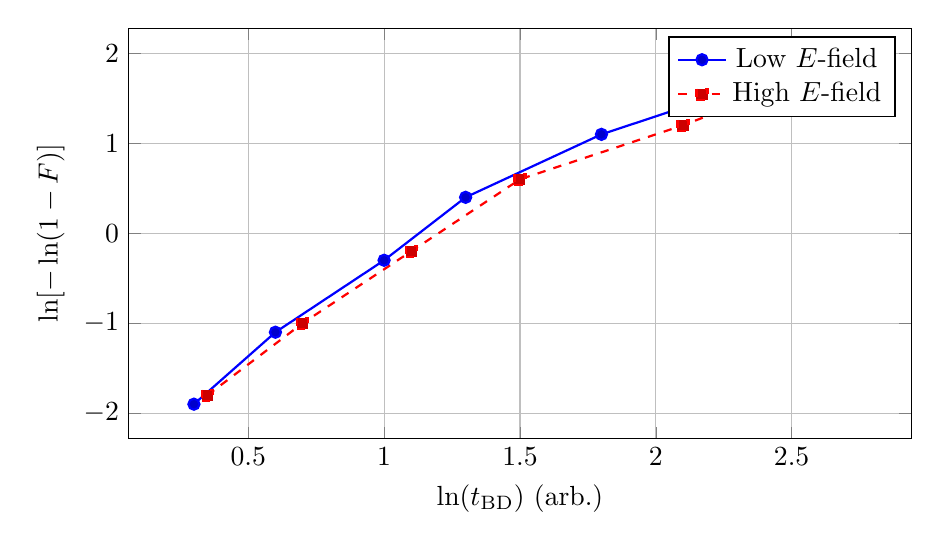
\begin{tikzpicture}
\begin{axis}[
  width=0.95\linewidth, height=0.56\linewidth,
  xlabel={$\ln(t_{\mathrm{BD}})$ (arb.)},
  ylabel={$\ln[-\ln(1-F)]$},
  grid=both, tick label style={/pgf/number format/fixed}
]
  \addplot+[mark=*, thick] coordinates
    {(0.30,-1.90) (0.60,-1.10) (1.00,-0.30) (1.30,0.40) (1.80,1.10) (2.30,1.60)};
  \addlegendentry{Low $E$-field}

  \addplot+[mark=square*, dashed, thick] coordinates
    {(0.35,-1.80) (0.70,-1.00) (1.10,-0.20) (1.50,0.60) (2.10,1.20) (2.70,1.90)};
  \addlegendentry{High $E$-field}
\end{axis}
\end{tikzpicture}
\caption{TDDB Weibull representation at two stress fields (illustrative).}
\end{figure}

\end{document}
